\documentclass[a4paper,12pt,french]{article}

\usepackage{../../Style}

\renewcommand\tabularxcolumn[1]{m{#1}}

\renewcommand{\baselinestretch}{1.25}

\newcommand{\canard}[3] {
\path [fill=black, fill opacity=0.3, draw=black, line width=2pt ] (#1,#2) -- (#1+1,#2+1) -- (#1+2,#2) -- (#1+8,#2+2) -- (#1+4,#2-2) -- (#1+7,#2-5) -- (#1+4,#2-4) -- (#1+3,#2-6) node[color=black,circle,minimum size=1pt,fill,inner sep=2pt,fill opacity=1] {} node[below right,fill opacity=1] {\textbf{{\Large{#3}}}} -- (#1+3,#2-3) -- (#1+1,#2) -- (#1,#2);
}

\pagestyle{empty}

\begin{document}
 
\begin{center}
\textbf{\huge{ Activité - Somme de vecteurs }}
\end{center} 

Un oiseau posé sur $A$ s'envole pour se poser en $B$. Après s'être reposé, il rejoint le point $C$.

\begin{center}
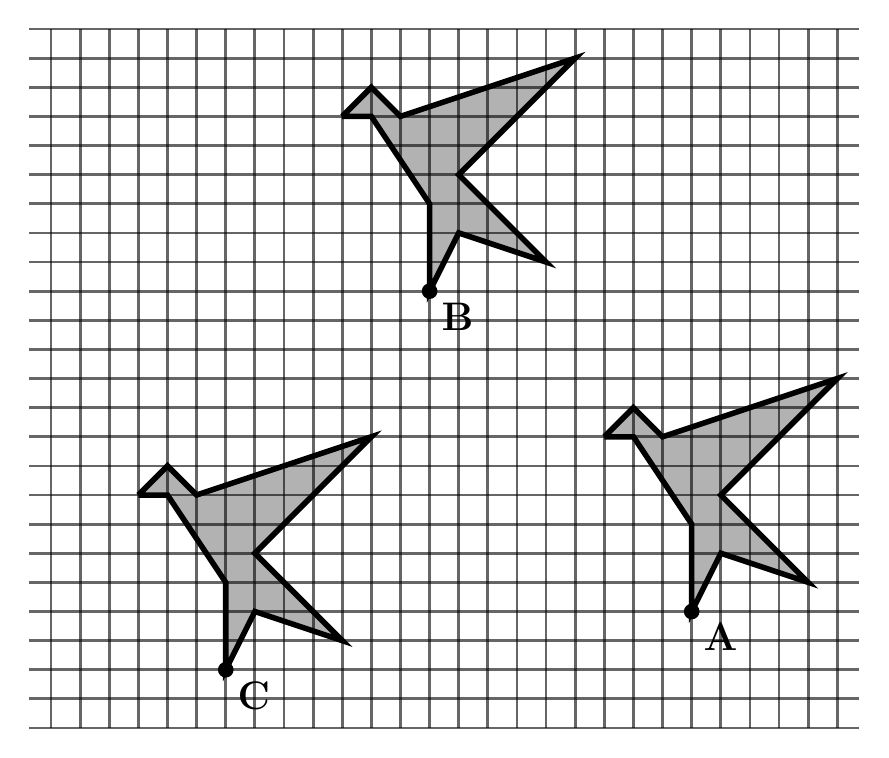
\begin{tikzpicture}[scale=1]
\begin{axis}[
%axis x line=bottom,
%axis y line = left,
%axis lines=middle,
width=\linewidth,
%height=0.8\linewidth,
xmin=3, xmax=28,
ymin=0, ymax=24,
%enlargelimits={abs=0.2},
xtick distance=1,
ytick distance=1,
grid=both,
xticklabels={},
yticklabels={},
grid style={black,line width=1pt, draw opacity=0.6},
ticks=none,
axis equal,
legend pos=north east,
axis line style={draw=none},
]
\canard {21} {10} A;
\canard {12} {21} B;
\canard {5} {8} C;
%\node[color=black,circle,minimum size=1pt,fill,inner sep=2pt,fill opacity=1,label={-45:\textbf{\Large B}}] at (15,15) {};
%\node[color=black,circle,minimum size=1pt,fill,inner sep=2pt,fill opacity=1,label={-45:\textbf{\Large C}}] at (8,2) {};

\end{axis}
\end{tikzpicture}
\end{center}

\begin{enumerate}

\item Dessiner l'oiseau après son premier déplacement et le vecteur qui symbolise ce mouvement.
\item Faire de même avec le deuxième déplacement.
\item Quel déplacement plus direct aurait pu effectuer l'oiseau pour arriver à sa position finale? Représenter le vecteur qui symbolise ce mouvement.

\item Compléter:

Effectuer la translation de vecteur $\vv {AB}$ suivie de la translation de vecteur $\vv {BC}$ revient à effectuer la translation de vecteur $\vv {AC}$.

\end{enumerate}

On peut alors définir la somme de deux vecteurs $\vv u$ et $\vv v$: $A$ étant un point quelconque, on place le point $B$ tel que $\vv {AB} = \vv u$ et $C$ tel que $\vv {BC} = \vv v$. Alors $\vv u + \vv v$ est le vecteur $\vv {AC}$.

On appelle cela la \textbf{relation de Chasles}:
$$\huge{\vv {A \textbf B} + \vv {\textbf BC} = \vv {AC}}$$

\end{document}
